\chapter{Architecture}
\section{Process architecture}
\begin{figure}[!htb]
    \centering
    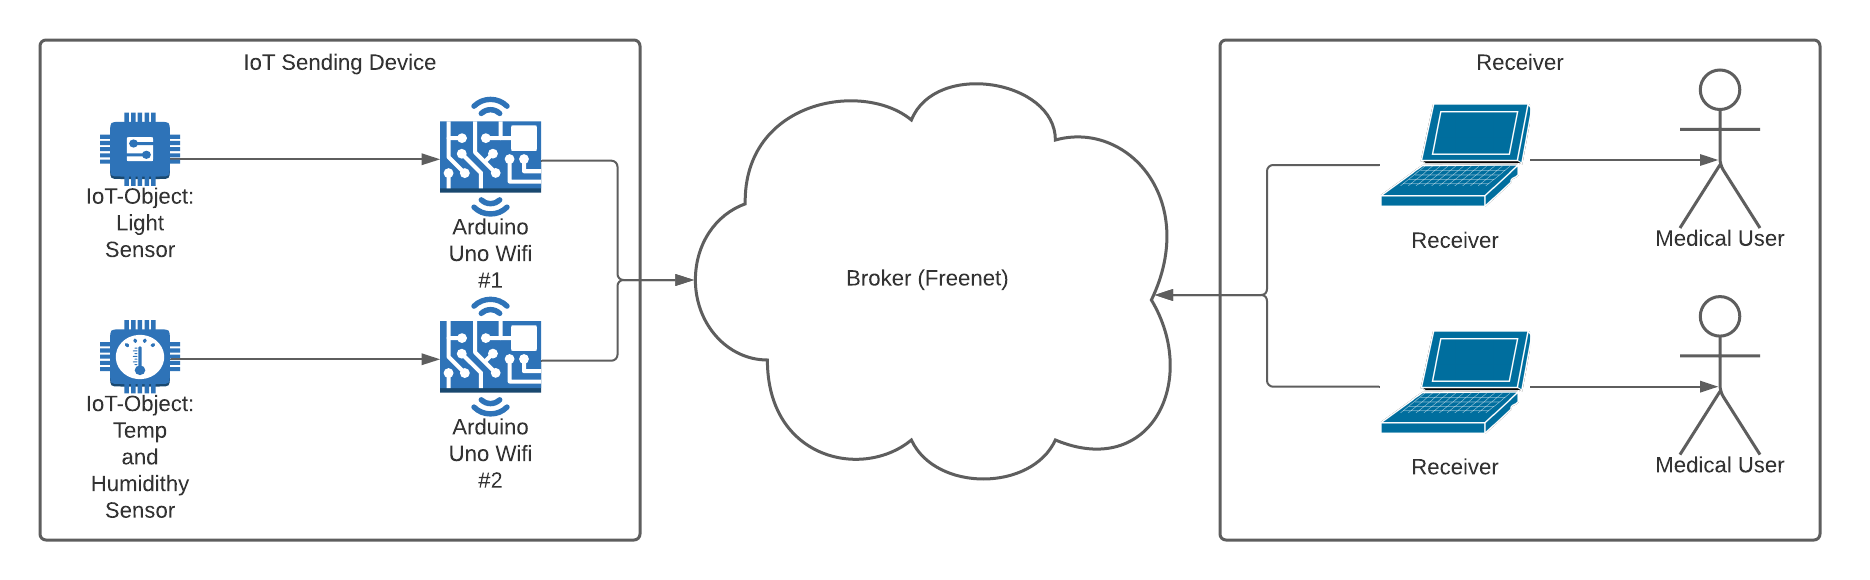
\includegraphics[width=15cm,height=19cm,keepaspectratio]{Architecture}
    \caption[Process overview]{Process overview}
    \label{fig:Architecture}
\end{figure}
\noindent
The figure above shows a complete process overview. Both endpoints are visible, on the left the IoT transmitter, the device that is with the patient and measures his vital signs. On the right is the endpoint device where the medical staff can evaluate the patient's values. The data exchange between the 2 endpoints takes place via a broker. In our architecture Freenet was used as broker. In order for the data to be transferred securely between the two endpoints, it must be protected from access and attack by third parties. This is done by an encryption between the two endpoints.
\newpage
\section{Arduino slot layout}
\begin{center}
\begin{figure}[!htb]
\subfigure{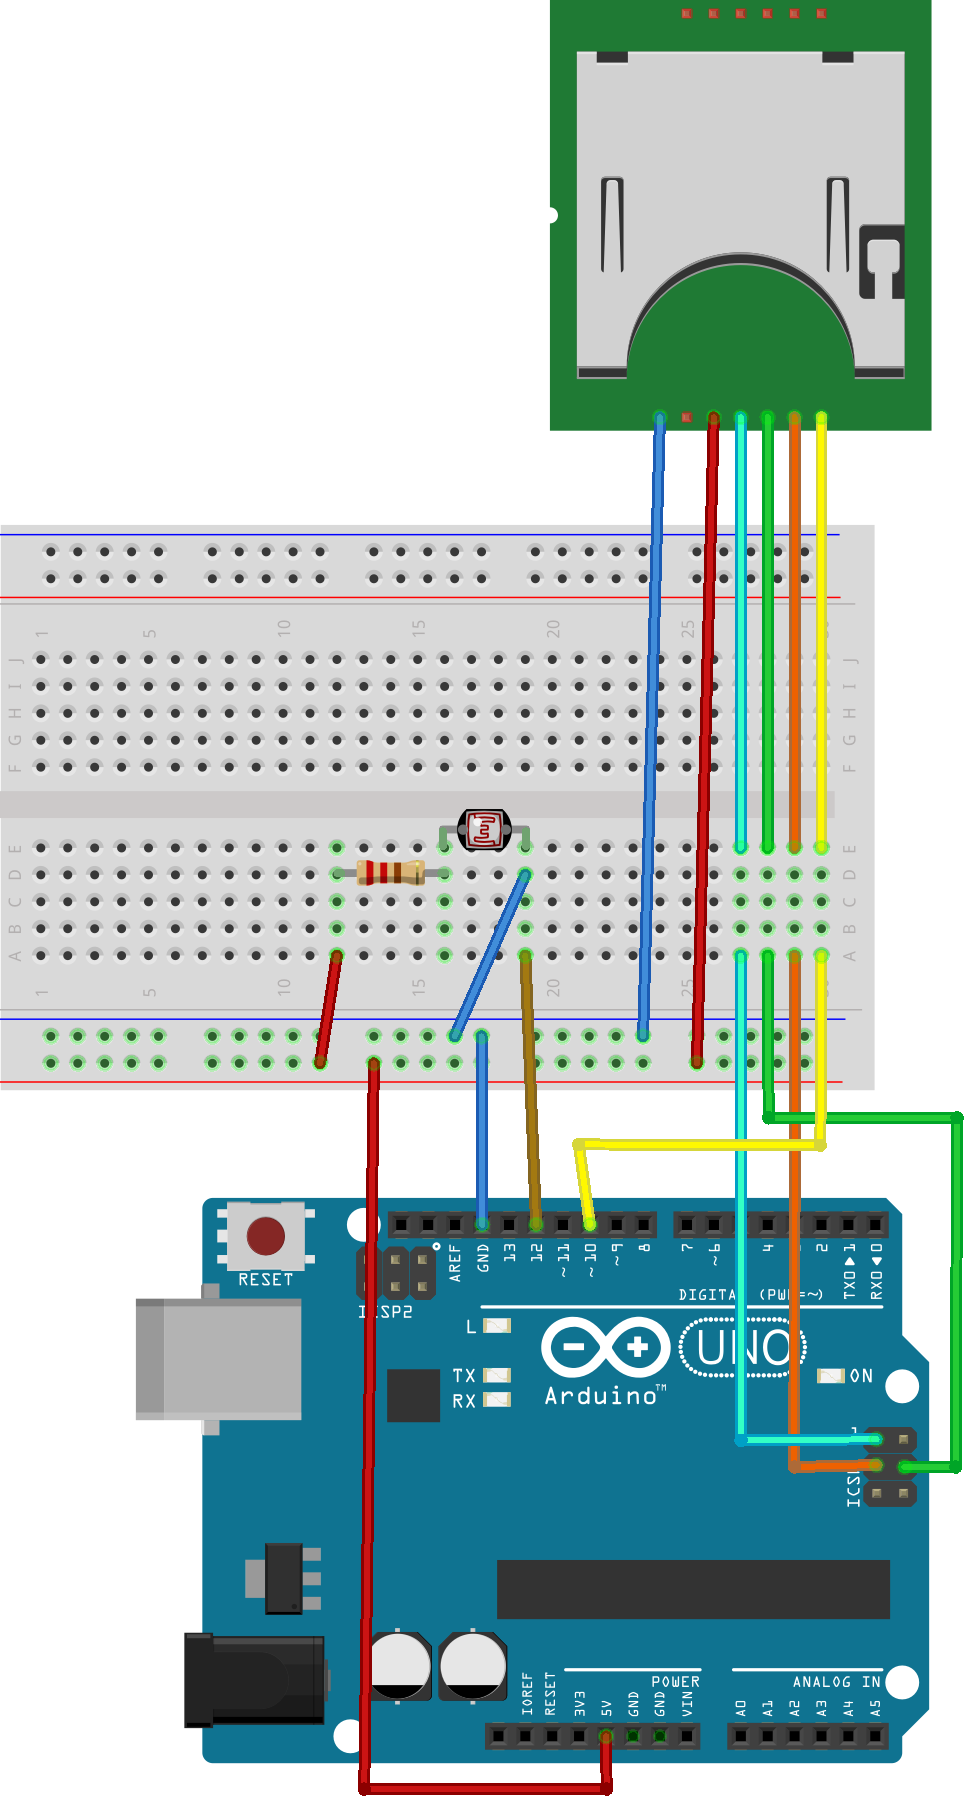
\includegraphics[width=6cm]{Arduino_LightSensor_Steckplatine}}
\hfill
\subfigure{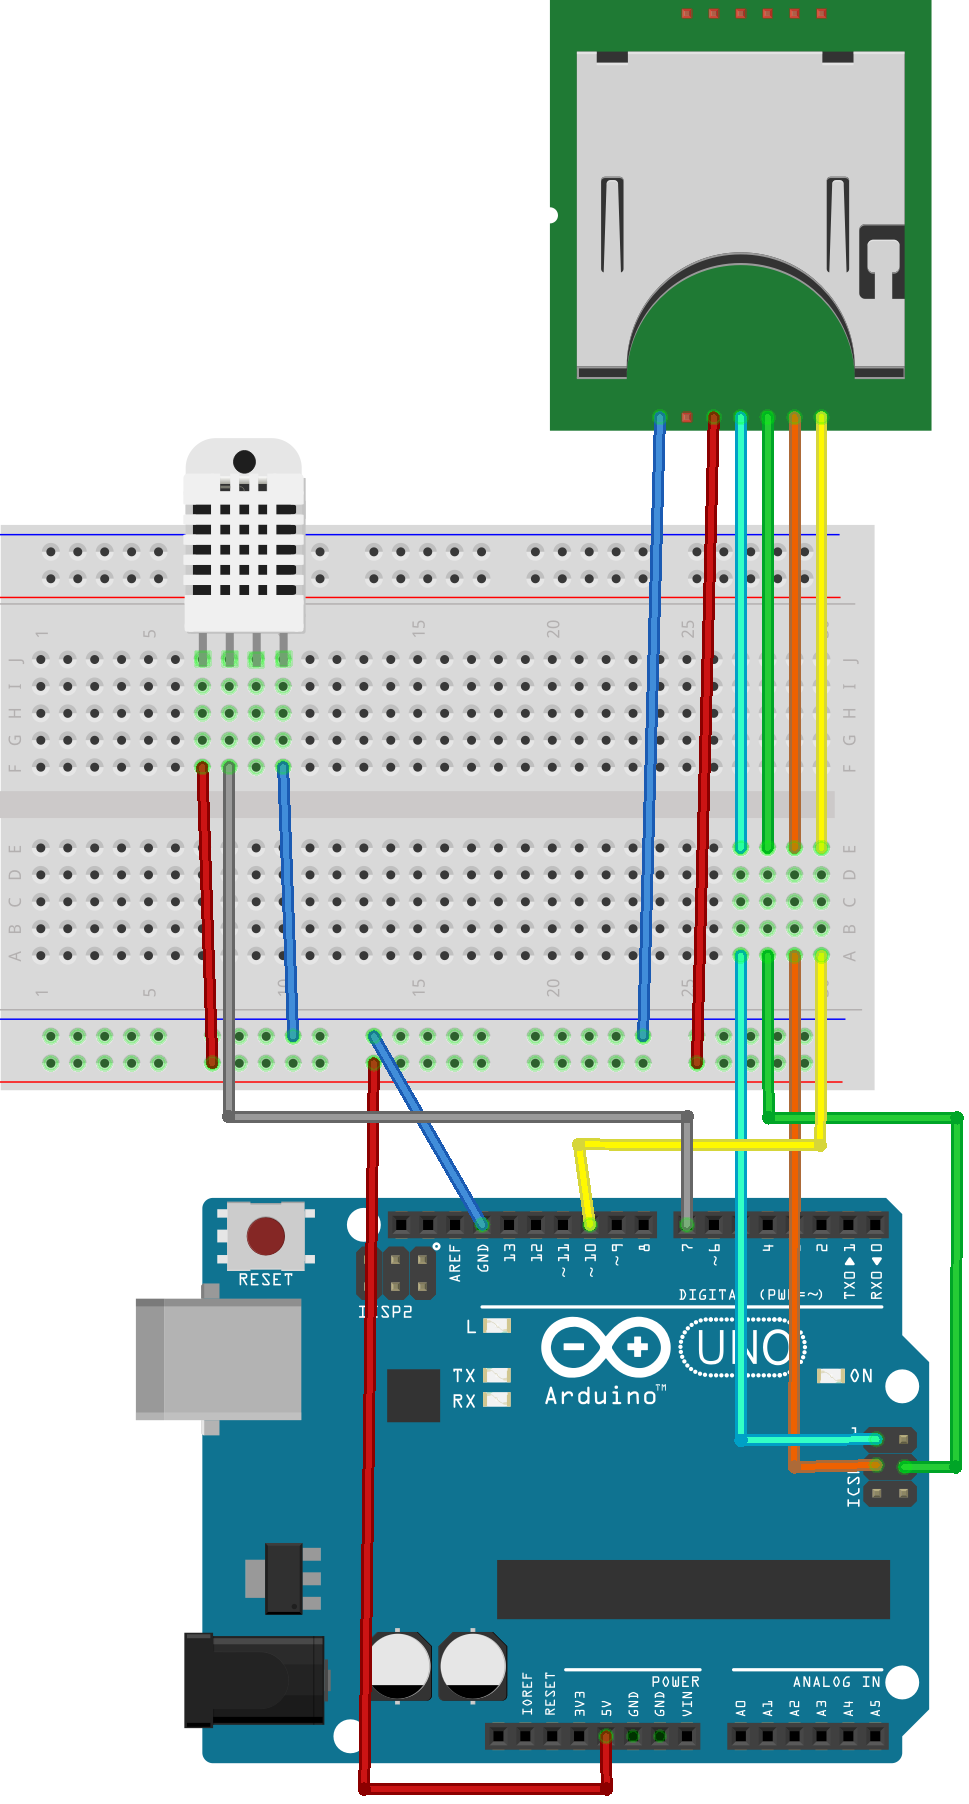
\includegraphics[width=6cm]{ArduinoTemp_Steckplatine}}
\caption{Arduino slot layouts}
\end{figure}
\end{center}
The two figures show an overview of the two Arduino cabling (IoT transmitter). The left figure shows the wiring with the light sensor and the right figure the wiring with the temperature sensor.
Bend Arduinos are also equipped with a micro SD card reader module, which is used to cache the communication data.
\newpage
\section{Preparations for initialization of communication}
In order for communication to occur between the two devices (sender and receiver), the two devices must exchange data over an insecure channel. Since the IoT devices are quite limited in terms of inputting data, they are equipped with a QR code. This QR code is scratchable, so that when the devices are received, it can be detected whether a QR code has already been read. The QR code contains a key that is used to send data to this device via Freenet. 
This initial data exchange takes place via an insecure channel. As soon as a recipient has registered with the sender via the QR code. A key exchange is executed via the insecure channel. In addition to the Key Exchange, new specific paths for the data exchange between the two devices are created and transmitted encrypted via the insecure channel. These new paths are then used for the subsequent data exchange.
\newpage